%%%%%%%%%%%%%%%%%%%%%%%%%%%%%%%%%%%%%%%%%%%%%%%%%%%%%%%%%
%%   $RCSfile: hpsg-include.tex,v $
%%  $Revision: 1.4 $
%%      $Date: 2007/05/27 13:27:12 $
%%     Author: Stefan Mueller (CL Uni-Bremen)
%%    Purpose: 
%%   Language: LaTeX
%%%%%%%%%%%%%%%%%%%%%%%%%%%%%%%%%%%%%%%%%%%%%%%%%%%%%%%%%
%% $Log: hpsg-include.tex,v $
%% Revision 1.4  2007/05/27 13:27:12  stefan
%% Umstellung auf Unicode + Fixes in Lokalitaet
%%
%% Revision 1.3  2006/05/17 12:19:27  stefan
%% *** empty log message ***
%%
%% Revision 1.2  2004/08/14 15:44:44  stefan
%% konstituentenreihenfolge
%%
%% Revision 1.1  2004/06/21 19:14:48  stefan
%% alte Version vor LaTeX-Beamer
%%
%% Revision 1.1  2003/04/22 10:13:29  stefan
%% Initial revision
%%
%% Revision 1.1  2001/10/21 17:01:35  stefan
%% Initial revision
%%
%%%%%%%%%%%%%%%%%%%%%%%%%%%%%%%%%%%%%%%%%%%%%%%%%%%%%%%%%

%% -*- coding:utf-8 -*-

%\includecomment{handout}
%\excludecomment{backup}
%\provideboolean{handout}\setboolean{handout}{true}


%\usepackage{epsfig}
%\usepackage{tabularx}

%% \usepackage{ifthen}


\selectlanguage{USenglish}

\usepackage{tikz}
\usetikzlibrary{patterns, matrix}


\usepackage{langsci-avm}

\let\mc=\multicolumn


%\usepackage{multimedia}

% \usepackage{media9}

% \newcommand{\includemovie}[3]{%
% \includemedia[%
% width=#1,height=#2,%
% activate=pagevisible,%
% deactivate=pageclose,%
% addresource=#3,%
% flashvars={%
% src=#3 % same path as in addresource!
% &autoPlay=true % default: false; if =true, automatically starts playback after activation (see option ‘activation)’
% &loop=true % if loop=true, media is played in a loop
% &controlBarAutoHideTimeout=0 %  time span before auto-hide
% }%
% ]{}{StrobeMediaPlayback.swf}%
% }% end of the new command


\title{Verbal reduplication in Mandarin Chinese: An HPSG account}

\author{Yanru Lu and Stefan Müller}

\institute[HU Berlin, Institute for German Language and Linguistics]{
  Institute for German Language and Linguistics, Syntax Lab\\
  Sprach- und literaturwissenschaftliche Fakultät\\
  HU Berlin% \\[2mm]
% St.Mueller@hu-berlin.de
}


\addbibresource{Bib.bib}

\begin{document}
\hypersetup{bookmarksopen=false}

\huberlintitlepage[22pt]

%\part{Einleitung}

\exewidth{(35)}


%%%%%%%%%%%%%%%%
%%%%%%%%%%%%%%% Intro
\section{Introduction}
\frame{
\frametitle{Verbal reduplication in Mandarin Chinese}

\begin{itemize}
\item<1-> In Mandarin Chinese, verbs can be reduplicated to express a delimitative aspectual meaning \citep[e.g.][]{Chao1968, Chen2001, Dai1997, Li1996, LiThompson1981, Tsao2001, XiaoMcEnery2004, Yang2003, Zhu1998}.
\item<2-> Delimitativeness: ``A short duration (i.e. transitoriness) and/or a low iteration frequency” \citep[155]{XiaoMcEnery2004}
  
\ea\label{ex:redup-ex} 
	\ea
	\gll qing ni chang zhe dao cai.\\
	please you taste this \textsc{clf} dish\\
	\glt `Please taste this dish.'
	
	\ex
	\gll qing ni \textbf{chang}-\textbf{chang} zhe dao cai.\\
	please you taste-taste this \textsc{clf} dish\\
	\glt `Please taste this dish a little bit.' 
	\z
\z

\item<3-> The current study tries to determine a suitable formal and unified analysis for the structure of verbal reduplication in Mandarin Chinese.

\end{itemize}
}


%%%%%%%%%%%%%%%%%
%%%%%%%%%%%%%%%% Phen
\section{The Phenomenon}


%%%%%%%%%%%%%%%%% Forms
\subsection{Forms}

\frame{
\frametitle{Forms}

\ea for monosyllabic verbs: \emph{shuo} `say'
		\ea \gll AA: shuo-shuo\\
		{} say-say\\
		\ex \gll A-\emph{yi}-A: shuo-yi-shuo\\
		{} say-one-say\\
		\ex \gll A-\emph{le}-A: shuo-le-shuo\\
		{} say-\textsc{pfv}-say\\
		\ex \gll A-\emph{le}-\emph{yi}-A: shuo-le-yi-shuo\\
		{} say-\textsc{pfv}-one-say\\
		\ex \gll AA-\emph{kan}: shuo-shuo-kan\\
		{} say-say-look\\
		\ex \gll A-\emph{kan}-\emph{kan}: shuo-kan-kan\\
		 {} say-look-look\\
		\z
\z
}

\frame{
\frametitle{Forms}

\ea \gll for disyllabic verbs: \emph{lai-wang}\\
	{} {} {} come-go\\
	\glt \hspace{1cm} `come and go/communicate'
		\ea \gll ABAB: lai-wang-lai-wang\\
		{} come-go-come-go\\
		\ex \gll AB-\emph{le}-AB: lai-wang-le-lai-wang\\
		{} come-go-\textsc{pfv}-come-go\\
		\ex \gll AABB: lai-lai-wang-wang\\
		{} come-come-go-go\\
		\z
\z
}

\frame{
\frametitle{Forms}

\ea \gll for V-O compounds: \emph{chang-ge} `sing'\\
	{} {} {} sing-song\\
		\ea \gll AAB: chang-chang-ge\\
		{} sing-sing-song\\
		\ex \gll A-\emph{yi}-AB: chang-yi-chang-ge\\
		{} sing-one-sing-song\\
		\ex \gll A-\emph{le}-AB: chang-le-chang-ge\\
		{} sing-\textsc{pfv}-sing-song\\
		\z
\z
}

\frame{
\frametitle{Forms}

\begin{itemize}
    \item There seems to be a fundamental difference between AA, ABAB and AABB \citep{Arcodiaetal2014, Fan1964, MelloniBasciano2018, Xie2020}.
    \item The current study will only focus on the AA, A-\emph{yi}-A, A-\emph{le}-A, A-\emph{le}-\emph{yi}-A and ABAB forms of verbal reduplication in Mandarin Chinese.
\end{itemize}
}


%%%%%%%%%%%%%%% distribution
\subsection{Syntactic distribution}

\frame{
\frametitle{Syntactic distribution}

\begin{itemize}[<+->]
\item Similar to an unreduplicated verb
\item Cannot combine with an expression of quantity.
\ea
    \ea[]{\gll ta yi tian pao shi li.\\
		he one day run ten mile\\
		\glt `He runs ten miles a day.'}
	\ex[*]{\gll ta yi tian \textbf{pao}-\textbf{pao} shi li.\\
	    he one day run-run ten mile\\}
    \z
\z
    \begin{itemize}
        \item Probably because the reduplication already contains a quantity meaning \citetext{\citealp[114--115]{Chen2005}; \citealp[84]{Li1998}}.
    \end{itemize}
\item Cannot combine with aspect markers other than \emph{le}.
\end{itemize}
}



%%%%%%%%%%%%%%%%%%% sem
\subsection{Semantics}

\frame{
\frametitle{Semantics}

\begin{itemize}[<+->]
    \item Core meaning: Delimitativeness
    \item A-\emph{yi}-A: Same core meaning as AA \citep{Fan1964, Yang2003}
    \item A-\emph{le}-A: Hierarchical combination of perfective and delimitativeness \citep[151]{XiaoMcEnery2004}
\end{itemize}
}

\frame{
\frametitle{Semantics}
\begin{itemize}[<+->]
    \item Incompatibility with aspect markers other than \emph{le} due to their semantics.
    \item Reduplication: holistic and dynamic viewpoint \citep{Dai1997, XiaoMcEnery2004}
    \begin{itemize}
        \item Holisticity: The situation as a non-decomposable whole
        \item Dynamicity: A process full of change
    \end{itemize}
    \item \emph{zhe} `\textsc{dur}', \emph{zai} `\textsc{prog}': Imperfective aspects \citep{XiaoMcEnery2004}
    \item \emph{guo} `\textsc{exp}': Change out of a state \citep{XiaoMcEnery2004}
    \item \emph{le}: Compatible with both changing process and changing point \citep{XiaoMcEnery2004}
\end{itemize}
}




%%%%%%%%%%%%%%%%
%%%%%%%%%%%%%% Prev
\section{Previous analyses}


\frame{
\frametitle{Previous HPSG analysis}

\begin{itemize}[<+->]
    \item \citet{FanSongBond2015}: Unified analysis for adjectival and verbal reduplication
    \item Adjectival reduplication: amplifier
    \item Verbal reduplication: downtoner
\end{itemize}

\begin{figure}
\centering
\begin{forest}
[\type{intensifier\_x\_rel}
 [\type{amplifier\_x\_rel}
  [\ldots]
  [\type{redup\_up\_x\_rel}]
 ]
 [\type{downtoner\_x\_rel}
  [\type{redup\_down\_x\_rel}]
  [\ldots]
 ]
]
\end{forest}
\caption{Type hierarchy for intensifier predicates according to \citet[100]{FanSongBond2015}}
\label{fig:fsb}
\end{figure}
}

\frame{
\frametitle{Previous HPSG analysis}

\begin{itemize}
    \item Reduplication is modeled as a lexical rule.
\end{itemize}

\ea\label{avm:fsb-redup}
\avm{
[\type*{redup-type}\\
cat|head & \1\\
val & \2\\
cont & \3 \normalfont \textsc{hook} [ltop & \4\\
			ind & \5]\\
c-cont & <[\type*{event-rel}\\
		pred & intensifier\_x\_rel\\
		lbl & \4\\
		arg1 & \5]>
]
}
$\to$
\avm{
[cat|head & \1\\
val & \2\\
cont & \3
]
}
\z
}

\frame{
\frametitle{Previous HPSG analysis}

\ea\label{avm:fsb-redup-a}
\avm{
[\type*{redup-a-lr $\subset$ redup-type}\\
cat|head & adjective\\
val & [spr <>]\\
c-cont & <[pred & redup\_up\_x\_rel]>
]
}\\
\textsc{orthography}: A $\to$ AA; (irregular AB $\to$ AABB)
\z

\ea\label{avm:fsb-redup-v}
\avm{
[\type*{redup-v-lr $\subset$ redup-type}\\
cat|head & verb\\
cont|hook & [aspect & non-aspect]\\
c-cont & <[pred & redup\_down\_x\_rel]>
]
}\\
\textsc{orthography}: A $\to$ AA; A $\to$ A-\emph{yi}-A; (irregular AB $\to$ ABAB)
\z
}

\frame{
\frametitle{Previous HPSG analysis}

\begin{itemize}[<+->]
    \item Advantages: 
    \begin{itemize}[<+->]
        \item Unified analysis for verbal and adjectival reduplication
        \item A-\emph{yi}-A as an alternative form of AA
    \end{itemize}
    \item Problems: 
    \begin{itemize}[<+->]
        \item A-\emph{le}-A is not possible because aspect markers are all blocked.
        \item ABAB and AAB are handled as irregular forms even though they are productive \citep{BascianoMelloni2017, MelloniBasciano2018, Xie2020, Xing2000stat}.
    \end{itemize}
\end{itemize}
}


%%%%%%%%%%%%%%%%%%%%%%
%%%%%%%%%%%%%%%%%%%%% current analysis
%%%%%%%%%%%%%%%%
%%%%%%%%%%%%%%% Analysis
\section{Current analysis}

\frame{
\frametitle{Verbal reduplication lexical rule}

\ea
\avm{
[\type*{verbal-reduplication-lr}\\
phon & \1 $\oplus$ \etag $\oplus$ \1\\
rels & \etag $\oplus$ \2 $\oplus$ < [\type*{delimitative-rel}\\
 	  arg \3 ] > \smallskip\\
lex-dtr & [phon \1\\
	synsem|loc & [cat|head & verb \\
                      cont|ind & \3 ]\\
        rels \2 ] ]
}
\z
}



\begin{frame}[fragile]
\frametitle{Type hierarchy for verbal reduplication and \emph{le}}

\begin{figure}
\centering
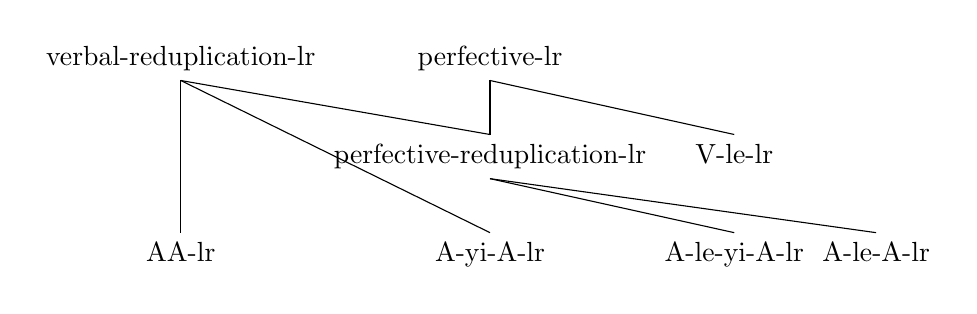
\begin{tikzpicture}

\matrix [matrix of nodes, row sep=0.7cm]
{
\node(redup){
	 \type{verbal-reduplication-lr}
	};
&
\node(le){
	\type{perfective-lr}
	};
\\
&
\node(1le31){
	\type{perfective-reduplication-lr}
	};
&
\node(vle){
	\type{V-le-lr}
	};
\\
\node(AA){
	\type{AA-lr}
	};
&
\node(AyiA){
	\type{A-yi-A-lr}
	}; 
&
\node(AleyiA){
	\type{A-le-yi-A-lr}
	};
&
\node(AleA){
	\type{A-le-A-lr}
	};\\
};

\draw (redup.south) -- (AA.north);
\draw (redup.south) -- (1le31.north);
\draw(redup.south) -- (AyiA.north);
\draw (le.south) -- (1le31.north);
\draw (1le31.south) -- (AleyiA.north);
\draw (1le31.south) -- (AleA.north);
\draw (le.south) -- (vle.north);

\end{tikzpicture}
\caption{Type hierarchy for lexical rules of verbal reduplication and \emph{le}}
\label{fig:typehi}
\end{figure}

\end{frame}



\frame{
\frametitle{Verbal reduplication lexical rule}

\ea\label{avm:AA}
\avm{
[\type*{AA-lr}\\
phon & \1 \+ \1\\
rels &  \2 $\oplus$ < [\type*{delimitative-rel}\\
 	  				arg & \3 ] >\\
lex-dtr & [phon & \1\\
	\punk{synsem|loc}{[cat|head & verb\\
                      cont|ind & \3]}\\
    rels & \2]
]
}
\z

\ea\label{avm:AyiA}
\avm{
[\type*{A-yi-A-lr}\\
phon & \1 \+ \phonliste{yi} \+ \1\\
rels &  \2 $\oplus$ < [\type*{delimitative-rel}\\
 	  					arg & \3 ] >\\
lex-dtr & [phon & \1\\
	\punk{synsem|loc}{[cat|head & verb\\
                      cont|ind & \3]}\\
    rels & \2]
]
}
\z
}

\frame{
\frametitle{Perfective lexical rule}

\ea\label{avm:pfv}
\avm{
[\type*{perfective-lr}\\
phon & \etag \+ \phonliste{le} \+ \etag\\
rels & <[\type*{perfective-rel}\\
       arg & \3]> \+ \2 \+ \etag\\
lex-dtr & [phon & \1\\
	\punk{synsem|loc}{[cat|head & verb\\
                      cont|ind & \3]}\\
        rels & \2]
]
}
\z

\ea\label{avm:vle}
\avm{
[\type*{V-le-lr}\\
phon & \1 \+ \phonliste{le}\\
rels & <[\type*{perfective-rel}\\
         arg & \3]> \+ \2\\
lex-dtr & [phon & \1\\
	\punk{synsem|loc}{[cat|head & verb\\
                      cont|ind & \3]}\\
        rels & \2]
]
}
\z

}

\frame{
\frametitle{perfective-reduplication-lr}

\ea\label{avm:pfv-redup}
\avm{
[\type*{perfective-reduplication-lr}\\
phon & \1 \+ \phonliste{le} \+ \etag \+ \1\\
rels & <[\type*{perfective-rel}\\
       arg & \3]>
       \+ \2 \+
        <[\type*{delimitative-rel}\\                 arg & \3]>\\
lex-dtr & [phon & \1\\
	\punk{synsem|loc}{[cat|head & verb\\
                      cont|ind & \3]}\\
    rels & \2]
]
}
\z

\ea\label{avm:AleyiA}
\avm{
[\type*{A-le-yi-A-lr}\\
phon & \1 \+ \phonliste{le, yi} \+ \1\\
lex-dtr & [phon & \1
                ]
]
}
\z

\ea\label{avm:AleA}
\avm{
[\type*{A-le-A-lr}\\
phon & \1 \+ \phonliste{le} \+ \1\\
lex-dtr & [phon & \1
                ]
]
}
\z
}


\frame{
\frametitle{Advantages of the current analysis}

\begin{itemize}
    \item Unified account for all forms of verbal reduplication in Mandarin Chinese (broader coverage than \citet{FanSongBond2015})
    \item A-\emph{yi}-A as alternative phonology of AA
    \item The form and the semantics of A-\emph{le}-A are correctly captured.
    \item Compatible with disyllabic verbs
    \item All productive forms are derivable from lexical rules.
\end{itemize}
}

\frame{
\frametitle{Summary}

\begin{itemize}
    \item Verbal reduplication in Mandarin Chinese is handled as a lexical rule.
    \item type hierarchy
    \item multiple inheritance
    
\end{itemize}
}



\appendix
% muss immer geladen werden, wegen Referenzen
%\input{hu-literatur-biber}

%\section<presentation>*{Literatur}

%% \frame{
%%   \frametitle<presentation>{Literatur}
  
%%   \beamertemplatebookbibitems

%% \bibliography{biblio}
%% \bibliographystyle{natbib.myfullname}
%% }
%\beamertemplatebookbibitems

% there seems to be a bug. These things are only set on the first literature slide
%
% The bug is still there, but the fix does not work any longer. 
\iflanguage{german}{\renewcommand{\refname}{Literaturverzeichnis}} % should be set automatically ???
%\iflanguage{german}{\def\insertsectionhead{Literaturverzeichnis}}{\def\insertsectionhead{\refname}}
\def\insertsectionhead{\refname}
\def\insertsubsectionhead{}

\huberlinjustbarfootline

\ifpdf
\else
\ifxetex
\else
\let\url=\burl
\fi
\fi
\begin{multicols}{2}
{\renewcommand*{\bibfont}{\tiny}

%\beamertemplatearticlebibitems

%\bibliography{bib-abbr,biblio,crossrefs}
%\bibliographystyle{unified}

% biblatex

%\addbibresource{bib-abbr.bib,biblio.bib}

% no book icon please
\setbeamertemplate{bibliography item}{}

%\printbibliography
\printbibliography[heading=bibliography,notkeyword=this] 

}
\end{multicols}



\end{document}


% Local variables:
% mode: lazy-lock
% End:
